\section{The PID Forms}
% \subsection{The PID Forms}

The PID controller are available on 3 main different form: Interactive, Non interactive (“standard”, “mixed” or sometimes “ideal) and Parallel.  

\textbf{The series form} sometime also call classical, real or interactive in equation [1] is the oldest controller used for direct field control which is either both of its input (PV) and output (MV) are directly connected to field or process equipment \cite{Wolfgang}. The original pneumatic and electronic controllers had this algorithm, and it is still found in many digital PID controllers today. The controller has been programmed to implement the interacting PID equation even though it is no longer an artifact of the hardware. The rationale for this programming is to have the digital controller behave identically to the legacy analog electronic or pneumatic controller it is replacing. This way, the proven tuning parameters of the old controller may be plugged into the new digital controller, yielding the same results.  
The famous Ziegler-Nichols PID tuning method was developed for this controller algorithm. 

\begin{figure}[H]
	\centering
	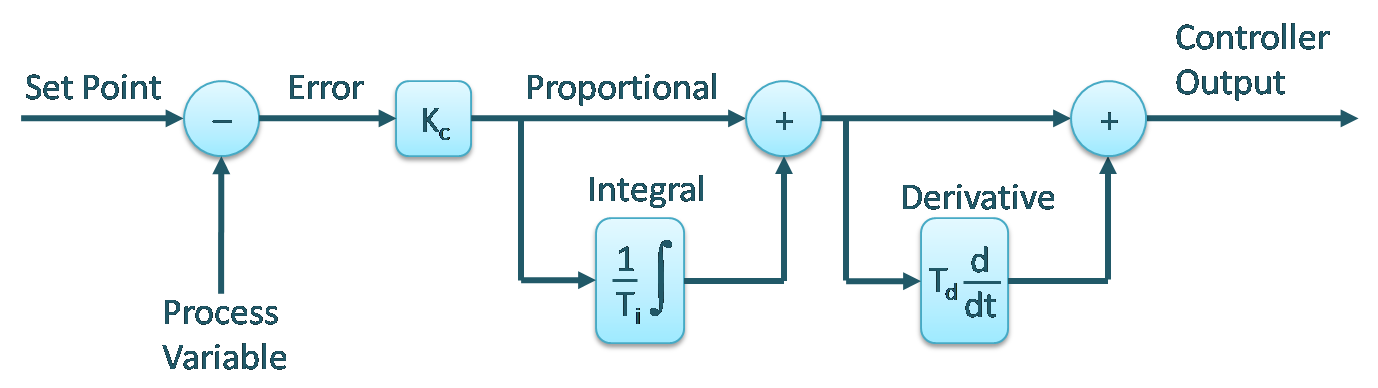
\includegraphics[width=0.8\columnwidth]{Pictures/series.png}
	\caption[Short title]{Serial form PID Controller \cite{PID}}
	\label{figure: Serial PID}
\end{figure}

\begin{equation}
\label{eqn:1}
    CO = K_c\cdot\left(e + \frac{1}{T_i}\int e\cdot dt \right)\cdot \left(1 + T_d\frac{de}{dt} \right)
\end{equation}


% A third version, with origins in the peculiarities of pneumatic controller mechanisms and analog electronic circuits, is called the Series or Interacting equation: 

% This “interacting” equation is an artifact of certain pneumatic and electronic controller designs. p Back when these were the dominant technologies, and PID controllers were modular designed such that integral and derivative actions were separate hardware modules included in a controller at additional cost beyond proportional-only action, the easiest way to implement the integral and derivative actions was in a way that just happened to have an interactive effect on controller gain. In other words, this odd equation form was a sort of compromise made for the purpose of simplifying the physical design of the controller. 

\textbf{The Ideal form} or non interactive algorithm is also called the standard or ISA algorithm. This form of controller is the classical teaching model of PID algorithms. It gives a clear understanding of P, I and D control, since: P-control, I-control and D-control can be seen independently of each other. Then, PID is effectively a combination of independent P, I and D-control actions. This can be seen in figure \ref{figure: Ideal PID}.
Since P, I and D algorithms are calculated independently in an ideal PID-controller. The Cohen-Coon and Lambda PID tuning rules were designed for this algorithm

\begin{figure}[H]
	\centering
	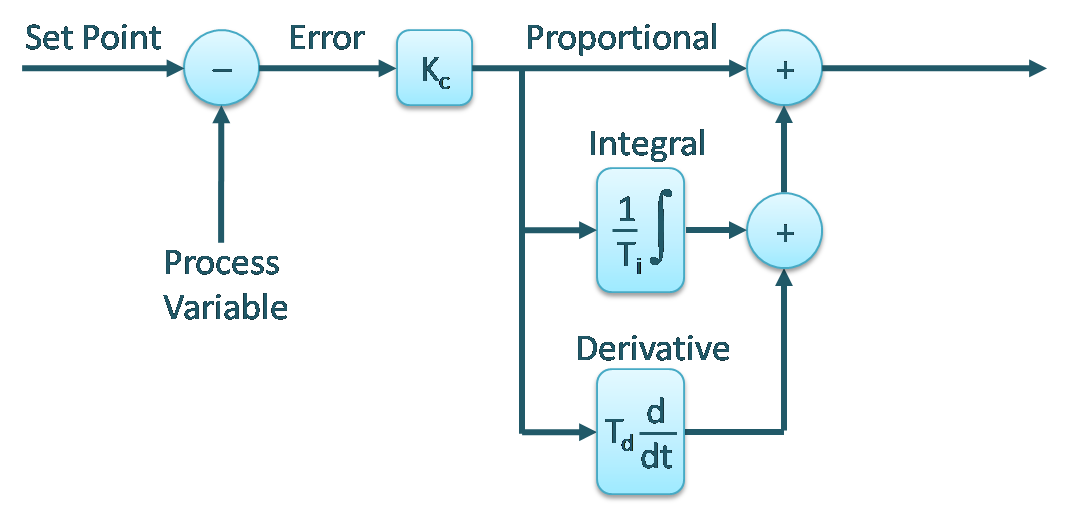
\includegraphics[width=0.8\columnwidth]{Pictures/ideal.png}
	\caption[Short title]{Ideal form PID Controller \cite{PID}}
	\label{figure: Ideal PID}
\end{figure}

\begin{equation}
\label{eqn:2}
    CO = K_c\cdot\left(e + \frac{1}{T_i}\int e\cdot dt +T_d\frac{de}{dt} \right)
\end{equation}

% An ideal process variable is a noise-free, refined and optimized variable. They are a result
% of computer optimization, process modeling, statistical filtering and value prediction
% algorithms

Note: If no derivative is used (i.e. Td = 0), the interactive and non interactive controller algorithms are identical. 

\textbf{The parallel form} has not often discussed in academic textbooks, but it is widely used nowadays in the  industry sector (distributes control system (DCSs) and PLCs application). This algorithm is simple to understand, but more difficult to tune. It has no controller gain affecting all three control modes (3 controller-action need to be tune separately), as a result it take more time to get the correct controller parameters. 

% Adjusting the proportional gain should be supplemented by adjusting the integral and derivative settings at the same time.

\begin{figure}[H]
	\centering
	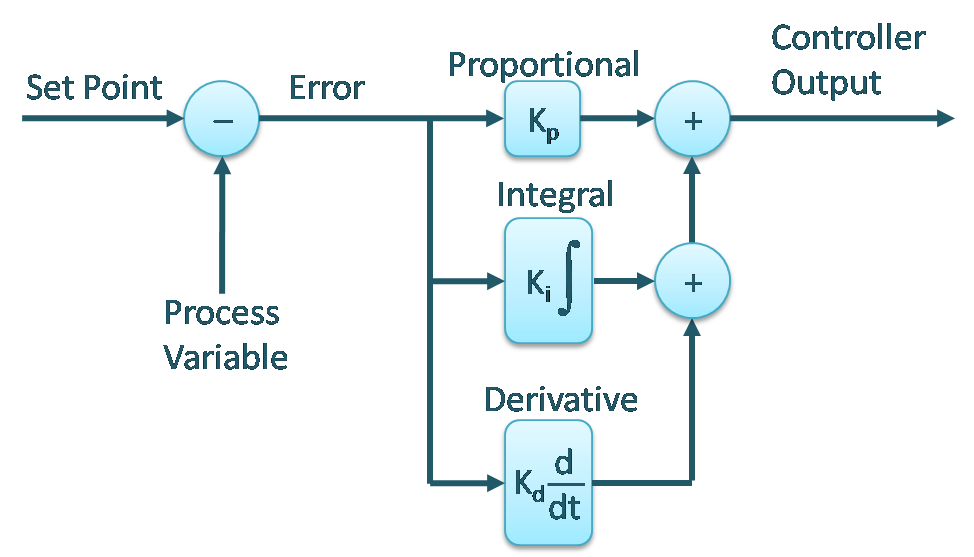
\includegraphics[width=0.8\columnwidth]{Pictures/parallel.png}
	\caption[Short title]{Parallel form PID Controller \cite{PID}}
	\label{figure: Parallel PID}
\end{figure}

\begin{equation}
\label{eqn:3}
    CO = K_p\cdot e + K_i\int e\cdot dt +K_d\cdot\frac{de}{dt}
\end{equation}

\textbf{Significance of Different Algorithms }

The biggest difference between the controller algorithms is that the parallel controller has a true proportional gain ($K_p$), while the other two algorithms have a controller Gain ($K_c$). The  $K_c$ Gain affects all three modes (Proportional, Integral and Derivative) of the Series and Ideal controllers, while $K_p$  affects only the proportional mode of a Parallel controller. 

This difference has a major impact on the tuning of the controllers. All the popular tuning rules (Ziegler-Nichols, Cohen-Coon, Lambda, and others) assume the controller does not have a parallel structure. 

% To tune a Parallel controller using any of these rules, the Integral time has to be divided and derivative time multiplied by the calculated Controller Gain. 

The second difference between the controller algorithms is the interaction between the \textbf{Integral} and \textbf{Derivative} modes of the Series (Interactive) controller. This is only of significance if the Derivative mode is used. In most PID controller applications, Derivative mode is not used  In practice D-action is not often used because of its sensitivity to the sensor noise. 

% Beyond the differences mentioned above, controllers also differ in the way the changes on controller output is calculated (positional and velocity algorithms), in the way Proportional and Derivative modes act on set point changes, in the way the Derivative mode is limited/filtered, as well as a interesting array of other minor differences. These differences are normally subtle, and should not affect your tuning. 

% To cut a long story short, it is hard to prescribe a particular form to implement a PID controller, each has its drawbacks and advantages. The standard structure is the most widespread in the field of industry. 
In the end, when tuning the controller, it is important to know what structure of the controller is (There are formulas to switch from one to another).


\newpage
